\chapter{Floating point data}

\hspace{4mm}Floating point data is a common way to store real numbers . Many different types of floating point data types exist, but the most relevant types for scientific computing are:

\begin{itemize}
    \item Double (FP64)
    \item Single (FP32)
    \item Half (FP16)
\end{itemize}

\begin{figure}[h!]
    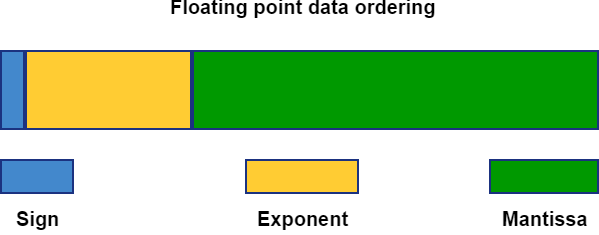
\includegraphics[width=0.6\linewidth]{figures/Float.png}
    \centering
    \caption{Floating point data structure.}
    \label{FP data}
\end{figure}

\vspace{5mm}

Floating point data contains three parts, the sign, the exponent and the mantissa. The sign and exponent are both stored as 2-base little-endian (most significant bit to the left) numbers. The mantissa is treated slightly differently. It is stored as a 2-base big-endian number (most significant bit to the right) with an implicit least significant bit equated to 0.

\subsection*{2-base number conversion}

Equation \ref{example binary eq.} provides an example conversion from the binary representation to the standard 10-base representation.

\begin{equation} \label{example binary eq.}
    \begin{split}
        \text{2 base sign/exponent} & = 0111 \\
        \text{10 base sign/exponent} & =  (8 \times 0) + (4 \times 1) + (2 \times 1) + (1 \times 1) =  7 \\
        \\
        \text{2 base mantissa} & = 0111 \\
        \text{10 base mantissa} & =  (1 \times 0) + (2 \times 0) + (4 \times 1) + (8 \times 1) + (16 \times 1) = 28 
    \end{split}
\end{equation}

\section{Calculating floating point value}

Equation \ref{FP formula eq.} provides the generic conversion formula for FP data. 

\begin{equation} \label{FP formula eq.}
    \text{Value} = -1^{Sign_{2}} \times 2^{Exponent_{10} - Bias_{10}} \times (1 + 1/(Mantissa_{10}))
\end{equation}

\noindent Bias is a data type specific number to "center" the exponent range around 0.

\subsection*{Double (64 bit)}

Common format for sensitive mathematical equations, like solving ill conditioned systems. It is also the default numerical data type of MATLAB.\autocite[]{wiki_double}

\begin{itemize}
    \item Bias: '1023'
    \item Sign: 1 bit
    \item Exponent: 11 bits
    \item Mantissa: 52 bits
    \item Resolution: $ (1/2)^{52} = 2.2204e-16 $
    \item Exponent range: $ 2^{([-1023,1024])} $
\end{itemize}

\subsection*{Single (32 bit)}

Original floating point data type used in 32 bit computers, provides sufficient resolution for many mathematical operations.\autocite[]{wiki_single}

\begin{itemize}
    \item Bias: '127'
    \item Sign: 1 bit
    \item Exponent: 8 bits
    \item Mantissa: 23 bits
    \item Resolution: $ (1/2)^{23} = 1.1921e-07 $
    \item Exponent range: $ 2^{([-127,128])} $
\end{itemize}

\newpage

\subsection*{Half (16 bit)}

Relatively coarse approximation of a real number, but sometimes good enough. A great example of applications that usually don't require more precision are  deep neural networks.\autocite[]{wiki_half}

\begin{itemize}
    \item Bias: '15'
    \item Sign: 1 bit
    \item Exponent: 5 bits
    \item Mantissa: 10 bits
    \item Resolution: $ (1/2)^{10} = 9.7656e-04 $
    \item Exponent range: $ 2^{([-15,16])} $
\end{itemize}

\vspace{5mm}

\newpage